\section{分离变量：把 PDE 还原为一族 ODE}
\label{sec:15-Differential-Equations-and-Dynamical-Systems/03-PDE-Introduction/04}

一根长 \(L\) 的细杆，两端浸在冰水里恒为零度，中段初始温度分布 \(u_0(x)\) 已知。前三节已经能说出解会越来越光滑、能量单调下降、时间不能倒着走——可要是有人问，二十秒后杆中点是几度，这些话一句也答不上来。定性判断到此为止，接下来需要一个能出数的办法。

\subsection{把解猜成乘积，方程就自己劈成两半}

要解的是

\[
\partial_tu=\kappa\,\partial_{xx}u,\qquad u(t,0)=u(t,L)=0 .
\]

直接积分走不通，因为等式两端一边是时间导数一边是空间导数，两个变量缠在一起。于是先退一步，只找那些形状特别简单的解：

\[
u(t,x)=T(t)X(x).
\]

这个试探并不假设所有解都长这样，它只是先攒一批特殊解，指望以后靠叠加拼出想要的那个。代入方程得到 \(T'X=\kappa TX''\)，在 \(T X\neq0\) 的地方两边同除 \(\kappa TX\)：

\[
\frac{T'(t)}{\kappa T(t)}=\frac{X''(x)}{X(x)} .
\]

左端只随 \(t\) 变，右端只随 \(x\) 变，而等式要对每一对 \((t,x)\) 都成立。固定 \(x\) 让 \(t\) 动，左端必须不动；固定 \(t\) 让 \(x\) 动，右端也必须不动。两边只能同时等于一个常数，记作 \(-\lambda\)，负号是事后诸葛亮，边界条件马上会逼着 \(\lambda\) 为正。一个 PDE 就此裂成两个 ODE：

\[
X''+\lambda X=0,\quad X(0)=X(L)=0;
\qquad
T'=-\kappa\lambda T .
\]

一个管空间形状，一个管时间演化，而且互不引用。第一单元处理过的常微分方程工具在这里全部可用。

\subsection{边界条件是一面筛子，只放行离散的一列频率}

先看空间那个。\(X''+\lambda X=0\) 是常系数二阶方程，通解的形态随 \(\lambda\) 的符号而变，逐一试过去就知道哪些 \(\lambda\) 能活下来。若 \(\lambda<0\)，通解是两个实指数的组合，代入 \(X(0)=X(L)=0\) 得到一个只有零解的齐次二元方程组。若 \(\lambda=0\)，通解是直线，两端为零同样只剩零解。若 \(\lambda>0\)，通解是 \(A\cos(\sqrt\lambda x)+B\sin(\sqrt\lambda x)\)，\(X(0)=0\) 杀掉余弦项，剩下的 \(X(L)=B\sin(\sqrt\lambda L)=0\) 要么 \(B=0\)（又是零解），要么 \(\sqrt\lambda L=k\pi\)。

于是非零解只在一列离散的 \(\lambda\) 上出现：

\[
\lambda_k=\Bigl(\frac{k\pi}{L}\Bigr)^2,
\qquad
X_k(x)=\sin\frac{k\pi x}{L},
\qquad k=1,2,3,\dots
\]

这些 \(\lambda_k\) 是算子 \(-\partial_{xx}\) 配上该边界条件后的特征值，\(X_k\) 是特征函数。方程本身对 \(\lambda\) 毫无挑剔，挑剔的是边界条件——只有恰好能在两端站住脚的波数被放行。矩阵的特征向量是被线性变换保持方向的向量（见\hyperref[sec:03-Linear-Algebra/05-Eigenvalues-and-Eigenvectors/01]{``不变方向与特征值：寻找矩阵最自然的坐标轴''}），这里的特征函数是被二阶导数算子保持形状的函数，两者是同一件事在有限维与无限维上的两个版本。

\subsection{每个频率按自己的时钟走，谁也不等谁}

时间那个方程简单得多。\(T'=-\kappa\lambda_kT\) 解出

\[
T_k(t)=e^{-\kappa\lambda_kt}=e^{-\kappa(k\pi/L)^2t} .
\]

第二节靠单频试探算出的 \(e^{-\kappa k^2t}\)，在这里作为完整推导的一部分重新出现。\(k=1\) 的最长波衰减最慢，\(k=10\) 的短波快一百倍。热方程的解越来越光滑，原因就摆在这一列指数里：粗糙对应高 \(k\)，高 \(k\) 先死。

\begin{center}
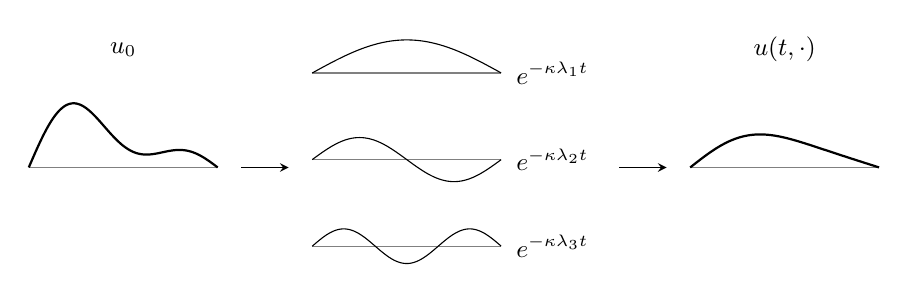
\begin{tikzpicture}[>=stealth]
  \begin{scope}[shift={(0,0.8)}]
    \draw[gray] (0,0) -- (2.4,0);
    \draw[thick] plot[domain=0:2.4,samples=120,variable=\x]
      ({\x},{0.5*(sin(75*\x)+0.6*sin(150*\x)+0.45*sin(225*\x))});
    \node at (1.2,1.5) {\small \(u_0\)};
  \end{scope}

  \draw[->] (2.7,0.8) -- (3.3,0.8);

  \begin{scope}[shift={(3.6,2.0)}]
    \draw[gray] (0,0) -- (2.4,0);
    \draw plot[domain=0:2.4,samples=80,variable=\x] ({\x},{0.42*sin(75*\x)});
    \node at (3.05,0) {\small \(e^{-\kappa\lambda_1t}\)};
  \end{scope}
  \begin{scope}[shift={(3.6,0.9)}]
    \draw[gray] (0,0) -- (2.4,0);
    \draw plot[domain=0:2.4,samples=100,variable=\x] ({\x},{0.28*sin(150*\x)});
    \node at (3.05,0) {\small \(e^{-\kappa\lambda_2t}\)};
  \end{scope}
  \begin{scope}[shift={(3.6,-0.2)}]
    \draw[gray] (0,0) -- (2.4,0);
    \draw plot[domain=0:2.4,samples=120,variable=\x] ({\x},{0.22*sin(225*\x)});
    \node at (3.05,0) {\small \(e^{-\kappa\lambda_3t}\)};
  \end{scope}

  \draw[->] (7.5,0.8) -- (8.1,0.8);

  \begin{scope}[shift={(8.4,0.8)}]
    \draw[gray] (0,0) -- (2.4,0);
    \draw[thick] plot[domain=0:2.4,samples=120,variable=\x]
      ({\x},{0.5*(0.78*sin(75*\x)+0.6*0.30*sin(150*\x)+0.45*0.05*sin(225*\x))});
    \node at (1.2,1.5) {\small \(u(t,\cdot)\)};
  \end{scope}
\end{tikzpicture}
\end{center}

\emph{初始剖面拆成一列正弦，每个分量按自己的指数速率缩小，再叠回来；中间那一列彼此不通消息。}

\subsection{叠加把一族特解拼成想要的那个解}

单个乘积解 \(u_k=X_kT_k\) 满足方程和边界条件，但它只携带一种空间频率，而真实的初始分布是各种频率的混合。线性方程在这里交出它的红利：满足方程与齐次边界条件的解，任意线性组合仍然满足。把所有 \(k\) 叠起来，

\[
u(t,x)=\sum_{k=1}^{\infty}b_k\sin\frac{k\pi x}{L}\;e^{-\kappa(k\pi/L)^2t}.
\]

令 \(t=0\) 就看出 \(b_k\) 该取什么：\(u_0(x)=\sum_kb_k\sin(k\pi x/L)\)，这是初始分布的正弦级数展开。正弦系在 \(L^2([0,L])\) 中是完备正交系（见\hyperref[sec:12-Real-Analysis-Support/07-Lp-Spaces-and-Function-Geometry/03]{``\(L^2\) 的几何让投影与正交可用''}），系数由正交投影一次算出：

\[
b_k=\frac{2}{L}\int_0^Lu_0(x)\sin\frac{k\pi x}{L}\,dx .
\]

至此上面那张图的三步全部落到公式上：左边是 \(u_0\)，中间是投影得到的一列系数各乘各的衰减因子，右边是求和。第二节那句``高频先死''现在成了可以代入数字的表达式——想知道二十秒后中点几度，取前十几项算个和就够，因为后面的项早被指数压到看不见。

严格来说，逐项求导与求和交换、级数按所需意义收敛，这些都需要条件。对光滑且满足相容性的初值，条件自然成立；对一般的 \(L^2\) 初值，级数在 \(L^2\) 意义下收敛，而``解''这个词的含义要等到下一节的弱解框架才说得清楚。

\subsection{换一个方程，机器照转，只有时间那一半换了零件}

同一套流程搬到波动方程 \(\partial_{tt}u=c^2\partial_{xx}u\) 上，空间部分一字不改——特征值问题只由算子和边界条件决定，与时间导数是几阶无关。变的是时间方程：

\[
T''+c^2\lambda_kT=0,
\qquad
T_k(t)=A_k\cos\frac{ck\pi t}{L}+B_k\sin\frac{ck\pi t}{L}.
\]

指数衰减换成了等幅振荡。每个空间频率对应一个独立的谐振子，初始位移定 \(A_k\)，初始速度定 \(B_k\)——第一节说波动方程要两组初始数据，账在这里对上了。``一根弦是无穷多个互不交换能量的弹簧''这句直觉，到此有了严格的写法。

矩形上的 Laplace 方程分离的则是两个空间变量：一个方向做特征展开，另一个方向解一族常系数二阶 ODE，两侧的边界值各定一半系数。没有时间，也就没有初值，两个边界把角色都担了。

\subsection{可分离的前提是几何与算子都足够对称}

分离变量看着像技巧，它的适用范围其实被三件事卡死。

首先必须线性且齐次。叠加原理是整台机器的发动机，非线性方程里乘积形式代进去之后除不干净，产不出两个独立的 ODE。源项与非齐次边界同样不在射程内，得先做齐次化变换，或者按特征函数展开把源项吸收进系数方程，或者改用 Green 函数。

其次区域要与坐标系相合。矩形配直角坐标、圆盘配极坐标、球体配球坐标时，坐标线贴着边界走，乘积试探才成立。区域一旦是 L 形或任意曲边，手算的特征函数不存在，只能求助数值特征展开或有限元。

第三，特征函数长什么样完全由几何决定。区间加齐次 Dirichlet 条件给正弦，加齐次 Neumann 条件给余弦，周期区间给完整的 Fourier 系（见\hyperref[sec:08-Numerical-Analysis/08-Fourier-and-Spectral-Methods/01]{``从 Fourier 级数到连续变换''}），圆盘的径向给 Bessel 函数，球面给球谐函数。换句话说，Fourier 展开并非从天而降的工具，它是分离变量在最对称的那种几何上的产物；换个几何，就换一族特殊函数。

计算上的延续是谱方法（见\hyperref[sec:08-Numerical-Analysis/08-Fourier-and-Spectral-Methods/04]{``谱方法：用光滑性换高精度''}）：既然解在特征函数基下的系数随 \(k\) 快速衰减，那就只留前 \(N\) 项，把 PDE 的时间推进变成 \(N\) 个标量 ODE 的推进。解足够光滑时，几十个基函数能顶得上有限差分上千个格点。反过来，解若带间断，系数衰减慢，截断会在间断附近留下振铃，这时谱方法就不是好选择。

四节走下来是一个闭环：认出方程类型，预判解的行为，用能量守住唯一与稳定，再在规则区域上把解算出来。剩下一个缺口——整条路线默认解可以逐点求导两次，而带尖角的波、带激波的流体明摆着做不到。下一节把方程的要求降到积分意义上，看看这个缺口怎么补。
